\section{Basic Definitions}
\label{sec:basic}

Formulas are built over a countable set of propositional variables
$\PV$, using the propositional connectives $\land$, $\lor$, $\to$, the
constant $\bot$ and the modal connectives $\Box$, $\Diam$.  We write
$\neg \varphi$ as a shorthand for $\varphi\to \bot$.  The symbols
$\land$, $\lor$ and $\to$ are also used to denote algebraic
operations.
The \emph{G\"odel algebra} is a structure
$\stru{[0,1],\land,\lor,\to}$ where:
\[
a\land b = \min(a,b)
\qquad
a \lor b = \max(a,b)
\qquad
a\to b =
\begin{cases}
  1 & \mbox{if $a\leq b$}\\
  b &  \mbox{if $a > b$}     
\end{cases}
\]

%% Gc-model
\noindent
 A \emph{\GM-model} (\emph{G\"odel  model}) $\M$ is a structure
 $\stru{W,R,e}$ where $W$ is a nonempty set (the set of worlds),
 $R$ is a map $W\times W\to [0,1]$ (the accessibility relation) and  $e : W \times \PV\to [0,1]$
 (the evaluation function).
If $R : W\times W\to \{0,1\}$, we say that $\M$ is \emph{crisp};
in this case,  $R \subseteq W\times W$. 
%We write $w_1 R w_2$ to mean that $(w_1,w_2)\in R$;
The map $e$ is extended to arbitrary formulas as follows:
\begin{itemize}
\item $e(w,\bot) = 0$;
\item $e(w,\a \star \b) = e(w,\a) \star e(w,\b)$, for $\star\in \{\,\land,\,\lor,\,\to\,\}$;
\item $e(w,\Box \a) = \inf_{w'\in W}  \{\,R(w,w') \to e(w',\a)  \,\}$;
\item $e(w,\Diam \a) =  \sup_{w'\in W}  \{\,R(w,w') \land e(w',\a)  \,\}$.
\end{itemize}


\noindent
Note that:
\[
 e(w,\neg\a) =
 \begin{cases}
   1 & \mbox{if $e(w,\a)=0$}    
   \\
   0 &   \mbox{if $e(w,\a)> 0$} 
 \end{cases}
 \qquad
 e(w,\neg\neg\a) =
 \begin{cases}
   1 & \mbox{if $e(w,\a) > 0$}    
   \\
   0 &   \mbox{if $e(w,\a)= 0$} 
 \end{cases}
\]
\noindent
A world $w'$ is an $R$-successor of $w$
iff  $R(w, w')>0$. If  $w_0$ has no $R$-successors,
then $e(w_0,\Box\a)=1$ and $e(w_0,\Diam\a)=0$, since
 $R(w_0,w') \to e(w',\a) = 1$ and $R(w_0,w')\land e(w',\a) = 0$
 for every $w'\in W$.
 A \GM-model $\M=\stru{W,R,e}$ is
\emph{witnessed} if the values of $e(w,\Box\a)$  and $e(w,\Diam\a)$  are witnessed by  some world $w'$ in $\M$,
namely:
\begin{itemize}
\item  $e(w,\Box \a)=r$ iff 
   there is $w'\in W$   such that  $R(w,w') \to e(w',\a) = r$;

\item if $e(w,\Diam \a)=r$ iff
   there is $w'\in W$  such that $R(w,w')\land e(w'\a) = r$.
  
\end{itemize}
As a consequence, in the definitions of $e(w,\Box \a)$ and  $e(w,\Diam \a)$,
the infimum and the superior are just the minimum and the maximum.
An example of  non-witnessed model is shown in Fig.~\ref{fig:nonWitn};
in the definition of $R$ and $e$ only the  non-zero values are displayed.
It holds that   $e(w_0,\Box p)=0$,  but there is no $w_j\in W$ such that
$R(w_0,w_j) \to e(w_j,p)=0$.
Note that  every finite \GM-model is witnessed. 



\begin{figure}[t]
  \centering
  \begin{minipage}{0.45\linewidth}
    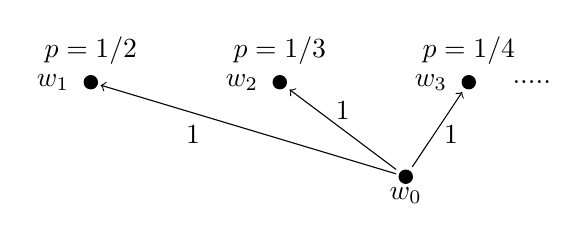
\begin{tikzpicture}[scale=0.8]
      % WORLDS  
      % w0
      \draw[fill] (0,-0.5) circle (3pt)
      +(0,-0)   node (w0)  {}  % used to label the circle 
      +(0,-0.3) node  {$w_0$}
      ;
      
      % w1 
      \draw[fill]  (-5,1) circle (3pt)
      +(0,0)   node (w1)  {}  % used to label the circle 
      +(-0.6,0)  node  {$w_1$} 
      +(0,0.5) node  {$p=1/2$}
      ;
      
      % w2
      \draw[fill] (-2,1) circle (3pt)
      +(0,0)   node (w2)  {}  % used to label the circle 
      +(-0.6,0) node{$w_2$}
      +(0,0.5) node{$p=1/3$}
      ;
      
      % w3
      \draw[fill] (1,1) circle (3pt)
      +(0,0)   node (w3)  {}  % used to label the circle 
      +(-0.6,0) node{$w_3$}
      +(0,0.5) node{$p=1/4$}
      ;
      
      % DOTS
      
      \draw[fill] (2,1) node{.....}  ; 
      
      % ARROWS
      \draw[->] (w0) -- (w1) node[midway,above, xshift=-2em,yshift=-2ex] {1};
      \draw[->] (w0) -- (w2) node[midway, above] {1}  ;
      \draw[->] (w0) -- (w3) node[midway, above, xshift=0.5em,yshift=-2ex] {1} ;
    \end{tikzpicture}
  \end{minipage}
      % -----------------------------------------      
      \fcolorbox{black}{gray!10}{
      \begin{minipage}{18em}\small
        \[
          \begin{array}{l}
            W=\{\,w_j~|~j\geq 0\,\}
\\[1ex]
            R(w_0,w_k)=1 \;\; k \geq 1
            \quad
            e(w_k,p) = \frac{1}{k+1}\;\; k\geq 1
          \end{array}
          \]
        \end{minipage}
      } % end box    
      % -----------------------------------------  
  $\small
    e(w_0,\Box p) \;=\; \inf_{j\geq 0}\{\,  R(w_0,w_j)\to e(w_j,p)  \,\}
    \;=\; \inf\{\;
 \overbrace{0\to 0}^1,\;\overbrace{1 \to (1/2)}^{1/2}, \; \overbrace{1 \to (1/3)}^{1/3}, \; \overbrace{1 \to (1/4)}^{1/4},  \,\dots  \;\}\;=\;0
  $
  \caption{A non-witnessed \GM-model $\M=\stru{W,R,e}$.}  
  \label{fig:nonWitn}
\end{figure}



A formula $\varphi$ is \emph{valid} in $\M=\stru{W,R,e}$ iff
$e(w,\varphi)=1$ for every world $w$ in $W$.  If $\varphi$ is not
valid in $\M$, we say that $\M$ is a \emph{countermodel} for
$\varphi$; thus, $\M$ contains a world $w$ such that $e(w,\varphi) <
1$.
A model $\M=\stru{W,R,e}$ is \emph{discrete} if $W$ is
finite and the images of $R$ and  $e$ are finite subsets of $\Qrange$, the set
of rational numbers in the range $[0,1]$.




Let  $\GL$ be the G\"odel-Dummett Logic, obtained by by extending
Intuitionistic Propositional Logic $\IPL$ with the linearity axiom
$(\a\to\b)\lor (\b\to \a)$.
%We recall the axiomatization of $\GCL$ given in~\cite{RodriguezV:21}.
G\"odel Modal Logic $\GKL$ is obtained by
adding to $\GL$ the following axioms and rules ($\vdash$ refers to
provability in $\GKL$):
\[
\begin{tabular}{m{3em}m{12em}m{3em}m{16em}}
  $(K_\Box)$ & $\Box(\a \to \b)\to (\Box\a\to \Box \b)$ & 
  $(K_\Diam)$ & $\Diam(\a \lor \b)\to (\Diam\a\lor \Diam \b)$
  \qquad $(F_\Diam)\; \neg \Diam\bot$ 
  \\
  $(FS_1)$ & $\Diam(\a \to \b)\to (\Box\a\to \Diam \b)$ & 
  $(FS_2)$ & $(\Diam \a \to\Box \b)\to \Box(\a\to  \b)$
  \\
  $(N_\Box)$ & $\vdash \a$ implies $\vdash \Box\a$ &
  $(N_\Diam)$ & $\vdash \a\to \b$ implies $\vdash \Diam \a\to\Diam\b$                                                   
\end{tabular}
\]
In~\cite{CaiRod2015} it is proved that  $\GKL$ is the set of formulas valid
in every  \GM-model.
We introduce some logics extending   $\GKL$, by providing a semantic characterization
(see Fig.~\ref{fig:diagram} for an overview):

\begin{itemize}
\item $\GCL$ is the set of formulas valid in every crisp \GM-model (see~\cite{RodriguezV:21});
\item  $\GWL$  is the set of formulas valid in every witnessed \GM-model;
\item $\GWCL$ is the set of formulas valid in every  witnessed crisp \GM-model (see~\cite{FerFioRod:2025}).
\end{itemize}


\noindent
The logic $\GCL$ is obtained by adding the axiom $\Box(\a\lor\b)\to (\Box \a \lor \Diam \b)$, we call $Cr$, 
to  $\GKL$ (see~\cite{RodriguezV:21}).
The logic $\GWCL$ has been introduced in~\cite{FerFioRod:2025} and no axiomatization is known.
By definition,  $\GKL\subseteq\GCL\subseteq\GWCL$ and $\GKL\subseteq\GWL\subseteq\GWCL$;
we show that all the inclusions are strict. 
Let   $\varphi =\Box (p\lor q)\to (\Box p \lor \Diam q)$  
and let $\M=\stru{W,R,e}$ be the  witnessed  $\GM$-model in Fig.~\ref{fig:countGW}.
Since $e(w_0,\varphi) = 0.6$, $\M$ is a countermodel for $\varphi$, and this certifies that
$\varphi\not\in\GWL$; accordingly, $Cr$ is not valid in $\GWL$.
Let  $Wt$ be the formula  $\Box \neg\neg \a\to \neg\neg \Box \a$;
we show that  $Wt$ is valid in  $\GWL$.
Let $\M=\stru{W,R,e}$ be a witnessed $\GM$-model and $w\in W$.
If $e(w, \neg\neg \Box \a)=1$, we immediately get $e(w, Wt)=1$. Otherwise,
 $e(w, \neg\neg \Box \a)=0$, hence $e(w, \Box \a)=0$.
Since $\M$ is witnessed,  there exists  $w'\in W$ such that $R(w,w') \to e(w',\a) = 0$;
it follows that   $e(w',\a)=0$, hence  $e(w',\neg \neg \a)=0$.
This implies  $e(w,  \Box\neg \neg  \a)=0$,
hence $e(w, Wt) = 1$. This proves  that
  $Wt$ is valid in $\GWL$.
Since  every finite model  is witnessed, 
   a countermodel for  $Wt$ must be infinite.
One can check that   the formula  $\varphi=\Box \neg\neg p\to \neg\neg \Box p$ 
is not valid in the infinite $\GM$-model $\M$ in Fig.~\ref{fig:nonWitn}, since  $e(w_0,\varphi) = 0$ (see, e.g.,~\cite{FerFioRod:2025}).
We point out that  $\M$  is crisp, accordingly $Wt$ is not valid in $\GCL$;
this also ascertains that  $\GCL$ has not the finite model property.

Finally, we stress  that, in all the mentioned modal logics, $\Box$ and $\Diam$ are not
interdefinable.
This is proved for  $\GCL$ in~\cite{RodriguezV:21};
in App.~\ref{app:noninterdBD} the proof is extended to all the other  modal logics mentioned above.





\begin{figure}[t]
  \centering
  

\begin{minipage}{\linewidth}
  \begin{center}
  \begin{tikzpicture}[
    level 1/.style={sibling distance=10em},
    % level 2/.style={sibling distance=4em},
    ]
    \node[fill=green!25] (GWc) {$\GWCL$}
    child{ 
      node[fill=green!25] (Gc) {$\GCL$}
      child[missing]{}
      child{
        node (GK)[fill=green!25]  {$\GKL$}
        edge from parent
        %node[right=.5ex] {$\subset$}
      } 
      edge from parent
      %node[right=.5ex] {$\subset$}
    }
    child{ 
      node[fill=green!25] (GW) {$\GWL$}
      edge from parent
      %node[left=.5ex] {$\subset$}
    } 
    ;

    

    %\draw (GW) -- node[left=.5ex] {$\subset$} (GK) ;    
    \draw (GW) -- (GK) ;    
    

    \node[right=1ex of GWc] {\begin{minipage}{16ex}
      \small (1), (2) valid\end{minipage}};
    \node[right=2ex of GW] {\begin{minipage}{16ex}
      \small (1) valid\par (2) NOT valid\end{minipage}};
    \node[left=-2ex of Gc] {\begin{minipage}{16ex}
      \small (1) NOT valid\par (2)  valid\end{minipage}};
    \node[right=1ex of GK] {\begin{minipage}{20ex}
      \small (1), (2) NOT valid\end{minipage}};

  \end{tikzpicture}
  \begin{minipage}{60ex}
    \begin{tabular}{p{30ex}p{50ex}}
      \begin{enumerate}[label=(\arabic*)]
      \item $\Box \neg\neg \a \to \neg\neg\Box \a$
      \item $\Box (\a \lor \b)\to (\Box \a \lor \Diamond \b)$
      \end{enumerate}
      &
      \begin{itemize}
      \item $\GCL = \GKL + (2)$ (see \cite{RodriguezV:21})
      \item $\GKL\subset\GCL\subset\GWCL$,   $\GKL\subset\GWL\subset\GWCL$
      \end{itemize}
    \end{tabular}
  \end{minipage}
\end{center}
\end{minipage}

%%% Local Variables: 
%%% mode: latex
%%% TeX-master: "goedelModalLogicWitnessNonCrisp"
%%% End: 

   \caption{Logics overview.}
  \label{fig:diagram}
\end{figure}


\begin{figure}[t]
  \centering
\[\small
  \begin{array}{c}
    \begin{minipage}{10em}
    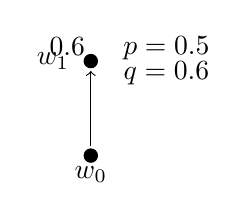
\begin{tikzpicture}[scale=0.8]
      % WORLDS  
      % w0
      \draw[fill] (0,0) circle (3pt)
      +(0,-0)   node (w0)  {}  % used to label the circle 
      +(0,-0.3) node  {$w_0$}
      ;
      
      % w1 
      \draw[fill]  (0,1.5) circle (3pt)
      +(0,0)   node (w1)  {}  % used to label the circle 
      +(-0.6,0)  node  {$w_1$} 
      +(1.2,0.2) node  {$p=0.5$}
      +(1.2,-0.2) node  {$q=0.6$}
      ;
      

      % ARROWS
      \draw[->] (w0) -- (w1) node[above left=-1.4] {0.6} ;
    \end{tikzpicture}
  \end{minipage}
  \begin{minipage}{20em}
    \[\small
    \begin{array}{l}
      % -----------------------------------------      
      \fcolorbox{black}{gray!10}{
        \begin{minipage}{15em}\small
          $W=\{\,w_0,\,\,w_1\,\}$
          \\[.5ex]
          $R(w_0,w_1) = 0.6$
          \\[.5ex]
          $e(w_1,p) = 0.5,\; e(w_1,q)=0.6$
        \end{minipage}
      } % end box    
      % -----------------------------------------  
    \end{array}
\]
  \end{minipage} 
\\[10ex]
    \begin{array}{rcl}
      e(w_0,\Box (p\lor q))&=&\inf\{\, R(w_0,w_0)\to e(w_0,p\lor q),\, R(w_0,w_1)\to e(w_1,p\lor q) \,\}\,=\,
\inf\{\, \overbrace{0\to 0}^1,\, \overbrace{0.6\to 0.6}^1 \,\}\,=\,1
    \\[0.5ex]
    e(w_0,\Box p) &=& \inf\{\, R(w_0,w_0)\to e(w_0,p),\,   R(w_0,w_1)\to e(w_1,p)\,\} \,=\,

              \inf\{\, \overbrace{0\to 0}^1,\,  \overbrace{0.6\to 0.5}^{0.5}\,\}    \,=\, 0.5
\\[0.5ex]
    e(w_0,\Diam q)&=& \sup\{\, R(w_0,w_0)\land e(w_0,q),\, R(w_0,w_1)\land e(w_1,q)\,\}\,=\,
\sup\{\, \overbrace{0\land 0}^0,\,  \overbrace{0.6\land 0.6}^{0.6}\,\}\,=\,  0.6
\\[1ex]
      e(w_0,\varphi) &=& e(w_0, \Box (p\lor q))\to e(w_0, \Box p \lor \Diam q) \,=\, 1\to   0.6 \,=\, 0.6
\end{array}
    \end{array}
  \]
  
  \caption{A countermodel  for the formula $\varphi=\Box (p\lor q)\to (\Box p \lor \Diam q) $.}
  \label{fig:countGW}
\end{figure}


\noindent






%%% Local Variables: 
%%% mode: latex
%%% TeX-master: "goedelModalLogicWitnessNonCrisp"
%%% End: 
